% !TeX root = ../main.tex
% !TeX program = xelatex
% !TeX encoding = UTF-8
\section{源—网—荷—储与建筑热状态的统一模型}

模型把资源可用量、设备与管网交付能力及建筑舒适要求共同约束，决定新增或退役容量和逐时运行量，并递推室温与储热量。功率采用kW，热量采用kWh，温度采用$^\circ$C，温差采用K；时间步长$\Delta t$采用h，连续案例取$1~\mathrm h$。

\begin{figure}[htbp]
\centering
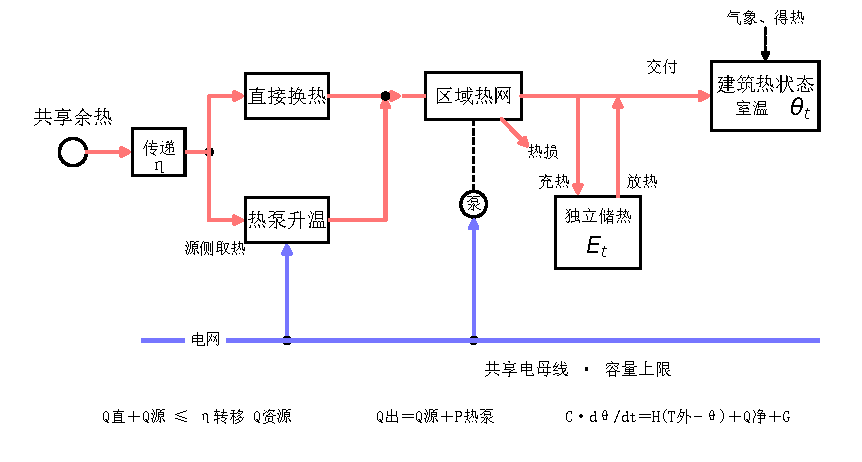
\includegraphics[width=\linewidth]{paper_r2/model_paper/source_network_load_storage_zh.pdf}
\caption{共享资源、热电网络与两类状态的统一结构。热泵源侧取热与电功分别计量；独立储热$E_t$与建筑室温$\theta_t$分别递推。各实验按配置启用模块。}
\label{fig:unified-structure}
\end{figure}

\subsection{资产容量与共享热资源}

温位表示用户所需的供水温度等级。同一设备向各温位的出力之和受可用容量限制。下文以$k,n,g,b,s,e,t$分别表示设备、区域节点、供热温位、建筑、储热装置、管段和时段。设备容量及出力满足
\begin{equation}
K_k=K_k^{\mathrm{exist}}+K_k^{\mathrm{new}}-K_k^{\mathrm{ret}},
\qquad
0\leq\sum_g Q_{k,g,t}\leq a_{k,t}K_k .
\label{eq:scoring-capacity}
\end{equation}
其中$K_k$为额定容量，三个上标分别表示现有、新增与退役容量；$Q_{k,g,t}$为向温位$g$供热的功率，$a_{k,t}$为逐时可用率。新增、退役、启停、最小出力及爬坡限制按设备配置设置。

直接换热与热泵共用余热时，须合计两类设备的取热量。热泵性能系数$\mathrm{COP}$为供热量与输入电量之比，其供热量扣除电功后才是源侧取热量。资源池$r$满足
\begin{equation}
R_{r,t}^{\mathrm{use}}
=\frac{1}{\eta_r^{\mathrm{tr}}}
\left[
\sum_{k\in\mathcal D_r,g}Q_{k,g,t}
+\sum_{k\in\mathcal H_r,g}
\left(1-\frac{1}{\mathrm{COP}_{k,g,t}}\right)Q_{k,g,t}
\right]
\leq \overline R_{r,t}.
\label{eq:scoring-resource}
\end{equation}
$R_{r,t}^{\mathrm{use}}$与$\overline R_{r,t}$分别为实际取用量和可用上限，$\eta_r^{\mathrm{tr}}\in(0,1]$为资源端至设备端的传热效率，$\mathcal D_r$与$\mathcal H_r$分别为直接换热和热泵设备集合。两类设备共用逐时资源限额，每个设备与资源池唯一关联，防止同一份余热被重复利用。资源传热、设备转换及管网输送的损失分别计算。

\subsection{设备性能域与温位适配}

通用模型按逐时工况给定$\mathrm{COP}$、制冷能效比$\mathrm{EER}$及转换效率；$\mathrm{EER}$为供冷量与输入电量之比。热泵与电锅炉分别满足
\begin{equation}
Q^{\mathrm{HP}}=\mathrm{COP}\,P^{\mathrm{HP}},\qquad
Q^{\mathrm{EB}}=\eta^{\mathrm{EB}}P^{\mathrm{EB}} .
\label{eq:scoring-conversion}
\end{equation}
其中$Q$为供热功率，$P$为输入电功率，上标$\mathrm{HP}$与$\mathrm{EB}$分别表示热泵和电锅炉，$\eta^{\mathrm{EB}}$为电锅炉效率。直接热源须满足用户供水温度要求；热泵升温后可接入更高温位。

设备性能域指厂家数据允许评价的工况范围。相应算例采用厂家表中同型号、同工况的供热功率$Q^{\mathrm{cat}}$与输入功率$P^{\mathrm{cat}}$，在相邻工况点间分别插值，再计算二者比值：
\begin{equation}
\begin{aligned}
Q_t^{\mathrm{cat}}&=\sum_i\lambda_{i,t}Q_i,\qquad
P_t^{\mathrm{cat}}=\sum_i\lambda_{i,t}P_i,\\
\mathrm{COP}_t^{\mathrm{cat}}&=\frac{Q_t^{\mathrm{cat}}}{P_t^{\mathrm{cat}}},\qquad
\lambda_{i,t}\geq0,\quad \sum_i\lambda_{i,t}=1 .
\end{aligned}
\label{eq:scoring-performance}
\end{equation}
其中$Q_i,P_i$为厂家表中工况点$i$的成对功率，$\lambda_{i,t}$由给定环境温度和出水温度确定。插值所需各点须有效且属于同型号，缺点、越界或跨型号组合不能参与优化。对工况有效的时段，固定整机算例以交付能力系数$\phi\in(0,1]$折减供热上限：
\begin{equation}
0\leq Q_t^{\mathrm{HP}}\leq\phi Q_t^{\mathrm{cat}},\qquad
P_t^{\mathrm{HP}}=
\frac{P_t^{\mathrm{cat}}}{\phi Q_t^{\mathrm{cat}}}Q_t^{\mathrm{HP}} .
\label{eq:scoring-duty}
\end{equation}
式\eqref{eq:scoring-duty}限定供热能力与单位耗电。理想小时占空比用小时内运行时间比例折算平均出力和耗电，不描述启停瞬态；型号、单位和工况随记录保存。

\subsection{节点守恒与网络物理反馈}

零失供时，节点按温位逐时平衡热源供热、管段输送、建筑用热和储热充放：
\begin{multline}
\sum_{k\in\mathcal K_n}Q_{k,g,t}
+\sum_{e\in\delta^-(n)}\eta_{e,t}F_{e,g,t}
+\sum_{s\in\mathcal S_{n,g}}Q_{s,t}^{\mathrm{dis}}\\
=D_{n,g,t}+\sum_{b\in\mathcal B_{n,g}}Q_{b,t}^{\mathrm h}
+\sum_{s\in\mathcal S_{n,g}}Q_{s,t}^{\mathrm{ch}}
+\sum_{e\in\delta^+(n)}F_{e,g,t}.
\label{eq:scoring-node}
\end{multline}
$\mathcal K_n$、$\mathcal S_{n,g}$和$\mathcal B_{n,g}$分别为相应设备、储热和建筑集合，$\delta^-(n)$与$\delta^+(n)$分别为流入和流出管段。$F$为管段入口功率，$\eta_{e,t}$为交付效率；$Q^{\mathrm{ch}}$与$Q^{\mathrm{dis}}$为充、放热功率，$Q_b^{\mathrm h}$为建筑实际受热功率。$D$只含建筑热状态模块未覆盖、且已计入需求侧调整的固定负荷，避免与建筑交付量重复计入。双向管段按实际方向计算，容量与改造状态限制输送，循环泵耗电计入系统电负荷。

热量够用还不代表远端供水温度和输送压力合格。对各支路独立设泵的星型管网，模型只采用有限个稳态模式；每个模式$m$给定流量和回水温度，并计算双管散热、水力阻力及泵功率：
\begin{equation}
\eta_m^{\mathrm{net}}=\frac{Q_m^{\mathrm{out}}}{Q_m^{\mathrm{in}}},
\qquad
P_m^{\mathrm{pump}}=
\frac{\Delta p_m\dot m_m}{1000\,\rho\,\eta_m^{\mathrm{pump}}}.
\label{eq:scoring-network}
\end{equation}
其中$Q_m^{\mathrm{in}}$与$Q_m^{\mathrm{out}}$为入口和出口热功率，其比值为输送效率；$\Delta p_m$为压差（Pa），$\dot m_m$为质量流量（kg/s），$\rho$为水密度（kg/m$^3$），$\eta_m^{\mathrm{pump}}$为泵效率，$P_m^{\mathrm{pump}}$为泵功率。求解后检查模式开启时的远端温度、流速、压降和泵功率，禁用不合格模式后重新求解。

\subsection{建筑热状态与精确逐时递推}

提前供热通过建筑蓄热影响后续室温，也增加散热。建筑采用1R1C结构\supcite{2}：等效热阻表示与室外的传热阻力，等效热容表示蓄热能力，室温是唯一状态。其变化满足
\begin{align}
C_b\frac{\mathrm d\theta_b}{\mathrm dt}
&=H_b(T^{\mathrm{out}}-\theta_b)+Q_b^{\mathrm h}-Q_b^{\mathrm c}+G_b,
\label{eq:scoring-rc-cont}\\
a_b&=\exp(-H_b\Delta t/C_b),\qquad
\beta_b=(1-a_b)/H_b,\\
\theta_{b,t}
&=a_b\theta_{b,t-1}+(1-a_b)T_t^{\mathrm{out}}
+\beta_b(Q_{b,t}^{\mathrm h}-Q_{b,t}^{\mathrm c}+G_{b,t}).
\label{eq:scoring-rc}
\end{align}
$\theta_b$为室温，$T^{\mathrm{out}}$为室外温度；$H_b$为围护与换气的总热损失系数（kW/K），$C_b$为等效热容（kWh/K）。$Q_b^{\mathrm h}$与$Q_b^{\mathrm c}$为供热和供冷功率，$G_b$为内部与太阳得热之和（kW）。$a_b$表示上一时段室温影响的保留程度，$\beta_b$表示净得热对室温的影响。式\eqref{eq:scoring-rc}是每时段输入保持不变时的精确积分，$\theta_{b,t}$为时段末室温。

室温受逐时舒适上下界约束，冷热受功率上限约束；启用互斥时，用二元变量排除同楼同时供热、供冷。建筑交付进入式\eqref{eq:scoring-node}，预热占用设备和配电容量，并增加散热。给定初温连续递推至规定终温或区间；方案比较固定舒适及初末态，避免透支末态蓄热，逐楼室温与交付量导出后复算。

给定目标室温时，可由式\eqref{eq:scoring-rc}反解所需净供热功率；本文在舒适带内联合选择室温与供热功率，使负荷随调度而变化。

\subsection{独立储热的连续性与边界}

独立储热以存量$E_{s,t}$表示，每时段扣损后加充热、减放热。以下$t=1,\ldots,T$，$E_{s,0}$为首小时开始前的存量，$K_s^E$为现有与新增能量容量，$r_s$为功率能量比（h$^{-1}$），则
\begin{align}
E_{s,t}
&=(1-\mu_s)^{\Delta t}E_{s,t-1}
+\eta_s^{\mathrm{ch}}Q_{s,t}^{\mathrm{ch}}\Delta t
-Q_{s,t}^{\mathrm{dis}}\Delta t/\eta_s^{\mathrm{dis}},
\label{eq:scoring-storage}\\
0\leq E_{s,t}&\leq K_s^E,\qquad
0\leq Q_{s,t}^{\mathrm{ch}},Q_{s,t}^{\mathrm{dis}}\leq r_sK_s^E .
\end{align}
$\mu_s$为每小时自损失率，$\eta_s^{\mathrm{ch}}$与$\eta_s^{\mathrm{dis}}$为充、放热效率；严格模式用二元变量约束充放互斥。$f_s^{\mathrm{init}}$与$f_s^{\mathrm{final}}$为初始和末端容量比例。固定初态采用$E_{s,0}=f_s^{\mathrm{init}}K_s^E$，组末要求$E_{s,\mathrm{end}}\geq f_s^{\mathrm{final}}K_s^E$；循环边界连接组首与组末。状态逐时递推，代表期权重只累计费用和能量，不放大状态变化。厂家与双楼机制实验不设独立储热，以识别建筑自身的调节作用。

\subsection{共享电力与多尺度耦合}

电驱热源、制冷设备和循环泵共用配电容量，其功率合计为系统电负荷：
\begin{align}
P_t^{\mathrm{sys}}
&=\sum_{k,g}\frac{Q_{k,g,t}^{\mathrm{HP}}}{\mathrm{COP}_{k,g,t}}
+\sum_k\frac{Q_{k,t}^{\mathrm{EB}}}{\eta_k^{\mathrm{EB}}}
\notag\\
&\quad+\sum_k\frac{Q_{k,t}^{\mathrm c}}{\mathrm{EER}_{k,t}}
+\sum_eP_{e,t}^{\mathrm{pump}},
\notag\\
(1+\sigma)P_t^{\mathrm{sys}}&\leq a_t^{\mathrm{grid}}K^{\mathrm{grid}}.
\label{eq:scoring-electric}
\end{align}
$P_t^{\mathrm{sys}}$为系统总电功率，$\sigma$为备用裕度，$K^{\mathrm{grid}}$为接入容量，$a_t^{\mathrm{grid}}$为逐时可用率。该式用于无微电网情形；启用微电网时，充电增加进口需求，本地发电与放电减少进口需求，进口须非负。系统接入容量限制区域合计电功率，区域节点向各楼交付热量，各楼室温约束所需冷热量。共享上限绑定时，一楼预热会减少其他楼的可用电功。

\subsection{费用与系统碳排放的统一核算}

费用和碳排放使用同一份调度量及时间权重。设$\omega_t=\pi_t w_t\Delta t$，其中$\pi_t$为情景概率，$w_t$为代表期对应的出现次数权重，核算式为
\begin{equation}
\begin{aligned}
C_0={}&\mathrm{CRF}\,I_{\mathrm{net}}+C_{\mathrm{fix}}+C_{\mathrm{event}}+C_{\mathrm{basic}}+C_{\mathrm{other}}
+\sum_t\omega_t\,\boldsymbol c_t^\mathsf T\boldsymbol x_t,\\
\mathcal E={}&\mathcal E_{\mathrm{const}}+\sum_t\omega_t\,\boldsymbol e_t^\mathsf T\boldsymbol x_t .
\end{aligned}
\label{eq:scoring-ledger}
\end{equation}
$C_0$为基本费用（元），$\mathcal E$为系统碳排放（kg），$\boldsymbol x_t$为逐时运行变量向量；$\boldsymbol c_t$与$\boldsymbol e_t$为相应费用和排放系数。$\mathrm{CRF}$为投资年化系数，将扣除补贴后的净投资$I_{\mathrm{net}}$折算为年费用；$C_{\mathrm{fix}}$为固定费用，其余费用项分别对应启停、基本电费及其他启用费用，$\mathcal E_{\mathrm{const}}$为排放常数项。后文采用$F_C=C_0+C_{\mathrm{carbon}}+C_{\mathrm{pref}}$、$F_E=\mathcal E$，其中新增项为碳费用与偏好惩罚。供热、供冷和共享电力的排放合计后受碳帽约束，即不得超过给定排放额度。

地源设备按地源$j$和情景累计供热取热量$E_j^{\mathrm{ext}}$与供冷排热量$E_j^{\mathrm{rej}}$，分别扣除与计入压缩机电耗。启用年度比例时，以$r_j^{\min}$与$r_j^{\max}$限制两者比例：
\begin{equation}
r_j^{\min}E_j^{\mathrm{rej}}\leq E_j^{\mathrm{ext}}
\leq r_j^{\max}E_j^{\mathrm{rej}} .
\label{eq:ground-ledger}
\end{equation}
